\documentclass{article} % For LaTeX2e
\usepackage{nips13submit_e,times}
\usepackage{hyperref}
\usepackage{epsfig}
%\usepackage{mahnig}
\usepackage{url}
\usepackage{enumerate}
\usepackage{booktabs}
%\documentstyle[nips13submit_09,times,art10]{article} % For LaTeX 2.09


\title{Shape classification using supervised classifiers}

\author{Julen Etxaniz and Ibon Urbina}

% The \author macro works with any number of authors. There are two commands
% used to separate the names and addresses of multiple authors: \And and \AND.
%
% Using \And between authors leaves it to \LaTeX{} to determine where to break
% the lines. Using \AND forces a linebreak at that point. So, if \LaTeX{}
% puts 3 of 4 authors names on the first line, and the last on the second
% line, try using \AND instead of \And before the third author name.

\newcommand{\fix}{\marginpar{FIX}}
\newcommand{\new}{\marginpar{NEW}}

\nipsfinalcopy % Uncomment for camera-ready version

\begin{document}

\maketitle

\begin{abstract}
  In this document we report our proposal for the application of supervised classification methods to the shape classification problem. The datasets we have selected are [plane and car shapes]. The classifiers that we have selected for the classification tasks were: [Linear discriminant analysis, Logistic regression, and Decision Trees]. We have implemented the classification process using the [scikit-learn and pandas library]. We have learned the classifiers using the train data and computing the accuracy in the test data. From our results the best accuracy has been produced by the [Logistic Regression Classifier].
\end{abstract}

\tableofcontents
\newpage

\section{Description of the problem}
The task we have to solve is the classification of the shape datasets, introduced in \cite{Thakoor:2007} \cite{Thakoor:2005-July} \cite{Thakoor:2005-Oct} and available from \url{http://biomecis.uta.edu/shape_data.htm}. 
 
There are 4 shape datasets available. We have selected the plane and car datasets. In each dataset, Cartesian coordinates of each point on the perimeter of each shape are stored as MATLAB data files named as $Class\%d\_Sample\%d.mat$.

\subsection{Plane dataset}

Shape database was created by taking 640X480 resolution pictures of replica models of airplanes from top.
The plane dataset has the following characteristics:

\begin{itemize}
    \item ? attributes.
    \item $7$ classes: (a) Mirage, (b) Eurofighter, (c) F-14 wings closed, (d) F-14 wings opened, (e) Harrier, (f) F-22, (g) F-15. See Figure \ref{fig:plane}.
    \item $210$ instances. 
    \item The data is perfectly balanced. There are 30 instances in each class.
\end{itemize}

\begin{figure}[ht]
    \centering
    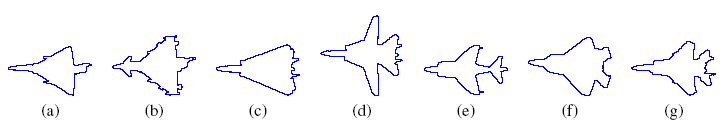
\includegraphics[width=\linewidth]{shape_plane.png}
    \caption{$7$ plane classes: (a) Mirage, (b) Eurofighter, (c) F-14 wings closed, (d) F-14 wings opened, (e) Harrier, (f) F-22, (g) F-15.}
    \label{fig:plane}
\end{figure}

\subsection{Car dataset}

Approach discussed in \cite{Thakoor:2005-Sept} was applied to 320X240 resolution videos to extract these shapes. As object extraction approach does not deal with shadows, the shapes are distorted in the bottom half. Samples show larger within-class variation, because vehicles of different makes and models vary.
The car dataset has the following characteristics:

\begin{itemize}
    \item ? attributes.
    \item $4$ classes: (a) Sedan, (b) Pickup, (c) Minivan, (d) SUV. See Figure \ref{fig:car}.
    \item $120$ instances. 
    \item The data is perfectly balanced. There are 30 instances in each class.
\end{itemize}

\begin{figure}[ht]
    \centering
    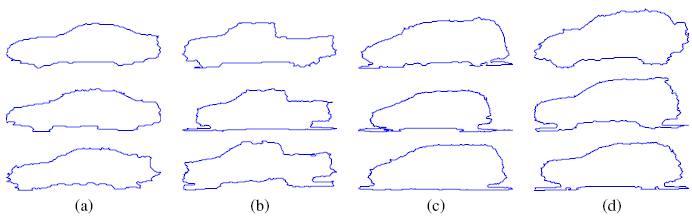
\includegraphics[width=\linewidth]{shape_car.png}
    \caption{$4$ car classes: (a) Sedan, (b) Pickup, (c) Minivan, (d) SUV.}
    \label{fig:car}
\end{figure}

\section{Description of our approach}
  
 We organized the implementation of the project according to the tasks:

\begin{enumerate} 

 \item Preprocessing of the dataset.

 \item Define and learn the classifiers using the training data.

 \item  Design the validation method to evaluate the accuracy of the proposed classification approaches.  
\end{enumerate} 


\subsection{Preprocessing}

  We used the pandas library to represent the dataset as a dataframe. We converted the values of the vehicle classes, that were represented as strings, to ordinal values between $0$ and $4$, because we have four classes.

  The data was split into two different sets: train and test, for validation. We use the same train set to learn all the classifiers, and the same test set for evaluating their accuracy.


\subsection{Classifiers}

 We use three different classifiers:

  \begin{enumerate}   
    \item Linear discriminant analysis with parameters:
       \begin{itemize}
           \item solver=’svd’ 
            \item shrinkage=None 
            \item priors=None 
            \item n\_components=None 
            \item store\_covariance=False 
           \item tol=0.0001
       \end{itemize}

    \item Logistic regression with parameters:
       \begin{itemize}
           \item penalty=’l2’
           \item dual=False
           \item tol=0.0001
           \item  C=1.0
           \item fit\_intercept=True
           \item intercept\_scaling=1
           \item class\_weight=None
           \item random\_state=None
          \item  solver=’liblinear’
          \item  max\_iter=100
          \item  multi\_class=’ovr’
          \item verbose=0, 
          \item warm\_start=False 
          \item  n\_jobs=1
       \end{itemize}
    \item Decision trees with parameters
      \begin{itemize}
           \item criterion=’gini’
           \item splitter=’best’ 
           \item max\_depth=None 
           \item min\_samples\_split=2
           \item min\_samples\_leaf=1 
           \item min\_weight\_fraction\_leaf=0.0 
           \item max\_features=None 
           \item random\_state=None 
           \item max\_leaf\_nodes=None 
          \item min\_impurity\_decrease=0.0 
          \item min\_impurity\_split=None 
          \item class\_weight=None 
          \item presort=False
       \end{itemize}
   \end{enumerate}

For each classifier, these were the parameters by default of the scikit-learn library\footnote{Hereyou should include the parameters of your implementation, not necessarily the default parameters of scikit-learn}. 
 
\subsection{Validation}
 
 To validate our results we compute the classifier accuracy in the test data. Another possibility was to compute the cross-validation in the complete dataset but we used the split between train and test because it was simpler. 

 As an additional validation step we computed the confusion matrices for the three classifiers.
 
\section{Implementation}

 All the project steps were implemented in Python. We used pandas for reading and preprocessing the dataset, and scikit-learn for the classification tasks. We illustrate how the implementation works in the Python notebook \texttt{Example\_Notebook\_Course\_Project.ipynb}.


\section{Results}

 The accuracies produced by the LDA, Logistic regression, and Decision tree classifiers were, respectively: $0.7068$, $0.7376$, and $0.6572$. Therefore, the best classifier was logistic regression.

 The results of the computation of the confusion matrices for  LDA, Logistic regression, and Decision tree classifiers are respectively shown in Tables~\ref{tab:CM_LDA}, \ref{tab:CM_LG}, and~\ref{tab:CM_DT}.

\begin{table}
\centering
\begin{tabular}{lrrrr}
\toprule \hline
col\_0 &   0 &   1 &   2 &   3 \\\hline
0     &  80 &   6 &   3 &   5 \\\hline
1     &   4 &  65 &   3 &  46 \\\hline
2     &   1 &   2 &  94 &   0 \\\hline
3     &   7 &  45 &   2 &  60 \\\hline
\bottomrule \hline
\end{tabular}
\caption{Confusion matrix produced by the LDA classifier}
 \label{tab:CM_LDA}
\end{table}

\begin{table}
\centering
\begin{tabular}{lrrrr}
\toprule\hline
col\_0 &   0 &   1 &   2 &   3 \\\hline
0     &  83 &   3 &   2 &   6 \\\hline
1     &   3 &  74 &   3 &  38 \\\hline
2     &   1 &   3 &  93 &   0 \\\hline
3     &   5 &  46 &   1 &  62 \\\hline
\bottomrule \hline
\end{tabular}
\caption{Confusion matrix produced by the Logistic regression classifier}
 \label{tab:CM_LG}
\end{table}

\begin{table}
\centering
\begin{tabular}{lrrrr}
\toprule \hline
col\_0 &   0 &   1 &   2 &   3 \\\hline
0     &  74 &   8 &   5 &   7 \\\hline
1     &   6 &  50 &   8 &  54 \\\hline
2     &   0 &   6 &  87 &   4 \\\hline
3     &   8 &  40 &   9 &  57 \\\hline
\bottomrule \hline
\end{tabular}
\caption{Confusion matrix produced by the Decision tree classifier}
 \label{tab:CM_DT}
\end{table}

The analysis of the confusion matrices shows that the most difficult discrimination, for all algorithms is between classes (1 and 3), which correspond to 'saab' and 'opel' vehicles. This occurs because the Saab 9000 and an Opel Manta 400 cars are more similar between them, than their difference to  a double decker bus or a  Cheverolet van. Therefore, even if the features are precise, they are not sufficient to make a good discrimination between these two vehicles. 

\section{Conclusions}
  In our project we have applied  [LDA, Logistic regression, and Decision tree classifiers] to the plane and car shape datasets, introduced in \cite{Thakoor:2007} \cite{Thakoor:2005-July} \cite{Thakoor:2005-Oct}. We have computed the accuracy of these classifiers and observed that [Logistic regression] produces the highest accuracy. We have also observed, from the analysis of the confusion matrices, that all classifiers make a poor discrimination between the Saab 9000 and an Opel Manta 400 cars. 


 \bibliographystyle{unsrt}
 \bibliography{bibtex_references_project}

\end{document}
